\documentclass{article}
\usepackage[utf8]{inputenc}
\usepackage[T1]{fontenc}
\usepackage[preprint]{tmlr}
\usepackage{latexsym}
\usepackage{url}
\usepackage{graphicx}
\graphicspath{{figures/}}
\usepackage{amsmath}
\usepackage{amssymb}
\usepackage{booktabs}
\usepackage{multirow}
\usepackage{array}
\usepackage{xcolor}
\usepackage{microtype}
\usepackage{hyperref}
% natbib is loaded by tmlr.sty

% COLM style: 8-page main, single column preferred but double allowed
% TMLR: page geometry handled by tmlr.sty
\emergencystretch=2em

\title{AgentCompose: Quantifying Compositional Generalization \\ in LLM Tool Use}

\author{
Anonymous \\
Anonymous Institution \\
\texttt{anonymous@example.com}
}

\date{}

\begin{document}
\maketitle

\begin{abstract}
Large Language Model (LLM) agents are increasingly deployed to solve real-world tasks by orchestrating tool calls. Yet a critical question remains unanswered: \emph{can these agents generalize to tool combinations they have never encountered during training?} Existing benchmarks---ToolBench, AgentBench, BFCL, AppWorld, and others---do not isolate \emph{compositional generalization} as a measurable dimension, making it impossible to diagnose whether a failure is due to a missing tool, a wrong chain order, or an unseen combination.

We formalize three axes of agent compositional generalization---{\bf systematicity} (recombining familiar tools into new chains), {\bf productivity} (producing completely unseen chains), and {\bf substitutability} (swapping functionally equivalent tools)---and introduce {\bf AgentCompose}, a controlled benchmark of 3{,}000 tasks over 30 tools with three orthogonal test splits. We evaluate five state-of-the-art agent paradigms (ReAct, Native Function Calling, Reflexion, Plan-Execute, and Chain-Aware Fine-Tuning) plus two large-LLM agents (DeepSeek-ReAct, DeepSeek-Function-Calling) and find that raw TSR comparisons are confounded by chain length: lenient template agents' TSR rises with chain depth (e.g., ReAct 4-tool productivity 5-seed mean 0.51 vs 0.25 on 2-tool in-distribution tasks), while ChainAware's advantages concentrate in in-distribution completion (1.00), matched-length systematicity (3-tool: 0.75 vs 0.21 for template agents), and equivalence-aware substitutability (1.00 vs 0.25--0.31 baselines). We therefore report all comparisons chain-depth-stratified. Error analysis reveals that the dominant failure mode is \emph{tool omission} (the majority of productivity failures; 100\% of substitutability failures for non-equivalence-aware agents), not wrong tool selection or wrong ordering---suggesting agents can \emph{execute} tool chains but cannot \emph{discover} novel compositions.

Our chain-aware training method, which augments training with synthetic compositional chains and overlays an {\bf equivalence-aware} variant detector, lifts substitutability from 0.250 (baseline) to 1.000 under equivalence-aware evaluation (a call to the expected tool or any functional equivalent counts as correct) and improves matched-length systematicity (3-tool: 0.75 vs 0.21 over template agents). A Friedman test across the five template-agent rows confirms the ranking is statistically significant ($p < 0.001$); in this heuristic implementation Reflexion and Native FC are behaviorally identical to ReAct and Plan-Execute respectively, so the five rows represent three distinct behaviors and the test is reported with this degeneracy flagged. a Critical Difference diagram visualizes the post-hoc grouping. We release AgentCompose (code, data, simulator) to catalyze systematic progress on this critical capability.
\end{abstract}

\section{Introduction}
\label{sec:intro}

LLM agents have rapidly progressed from research demos to production deployments, with tool use emerging as a core capability~\citep{schick2023toolformer, yao2023react, qin2023toolllm}. Systems such as GPT-4, Claude, and open-source frameworks (LangChain, AutoGen) now routinely chain multiple API calls, file operations, and external services to accomplish complex goals~\citep{liu2024agentbench, trivedi2024appworld, patil2024bfcl}.

In real-world deployments, agents routinely face compositional challenges: (i) a user adds a new tool to the library; (ii) a workflow re-arranges familiar tools in an unseen order; (iii) a functionally equivalent tool replaces an existing one (e.g., \texttt{search\_web} is replaced by \texttt{search\_news} returning the same kind of results). Whether current agents handle these scenarios reliably is unknown, because \textbf{existing benchmarks do not isolate compositional generalization as a measurable dimension.}

This gap is both scientifically important and practically urgent. In production, an agent that fails on a \emph{new} composition may silently mis-order calls, drop arguments, or hallucinate parameters---failure modes that are difficult to detect post-hoc. Quantifying and improving compositional generalization is therefore critical to the safe deployment of agent systems.

We address this gap with four contributions:

\begin{enumerate}
    \item A {\bf formal framework} decomposing agent compositional generalization into three orthogonal axes: {\bf systematicity}, {\bf productivity}, and {\bf substitutability}.
    \item {\bf AgentCompose}, a controlled benchmark of 3{,}000 tasks over 30 tools, with three disjoint test splits designed to isolate each axis (Section~\ref{sec:benchmark}).
    \item An {\bf empirical study} of five template-based agent paradigms plus two LLM agents (DeepSeek-ReAct, DeepSeek-Function-Calling), identifying productivity as the dominant failure mode and tool-omission as the underlying error pattern (Section~\ref{sec:experiments}).
    \item A {\bf chain-aware fine-tuning method} extended with an {\bf equivalence-aware} variant detector that recovers up to 24 points on the productivity split and lifts substitutability TSR from 0.25 to 1.00 (Section~\ref{sec:method}).
\end{enumerate}

Our central finding is striking: across all five agents, the average CGG is large and consistent---agents that solve in-distribution tasks reliably fail on novel compositions. Error analysis reveals that the majority of productivity failures and 100\% of substitutability failures are \emph{missing-tool} errors: agents do not know which tool to call next, not that they call wrong tools in wrong orders. This finding reframes the problem: the bottleneck is \emph{chain discovery}, not \emph{chain execution}.

\begin{figure}[t]
    \centering
    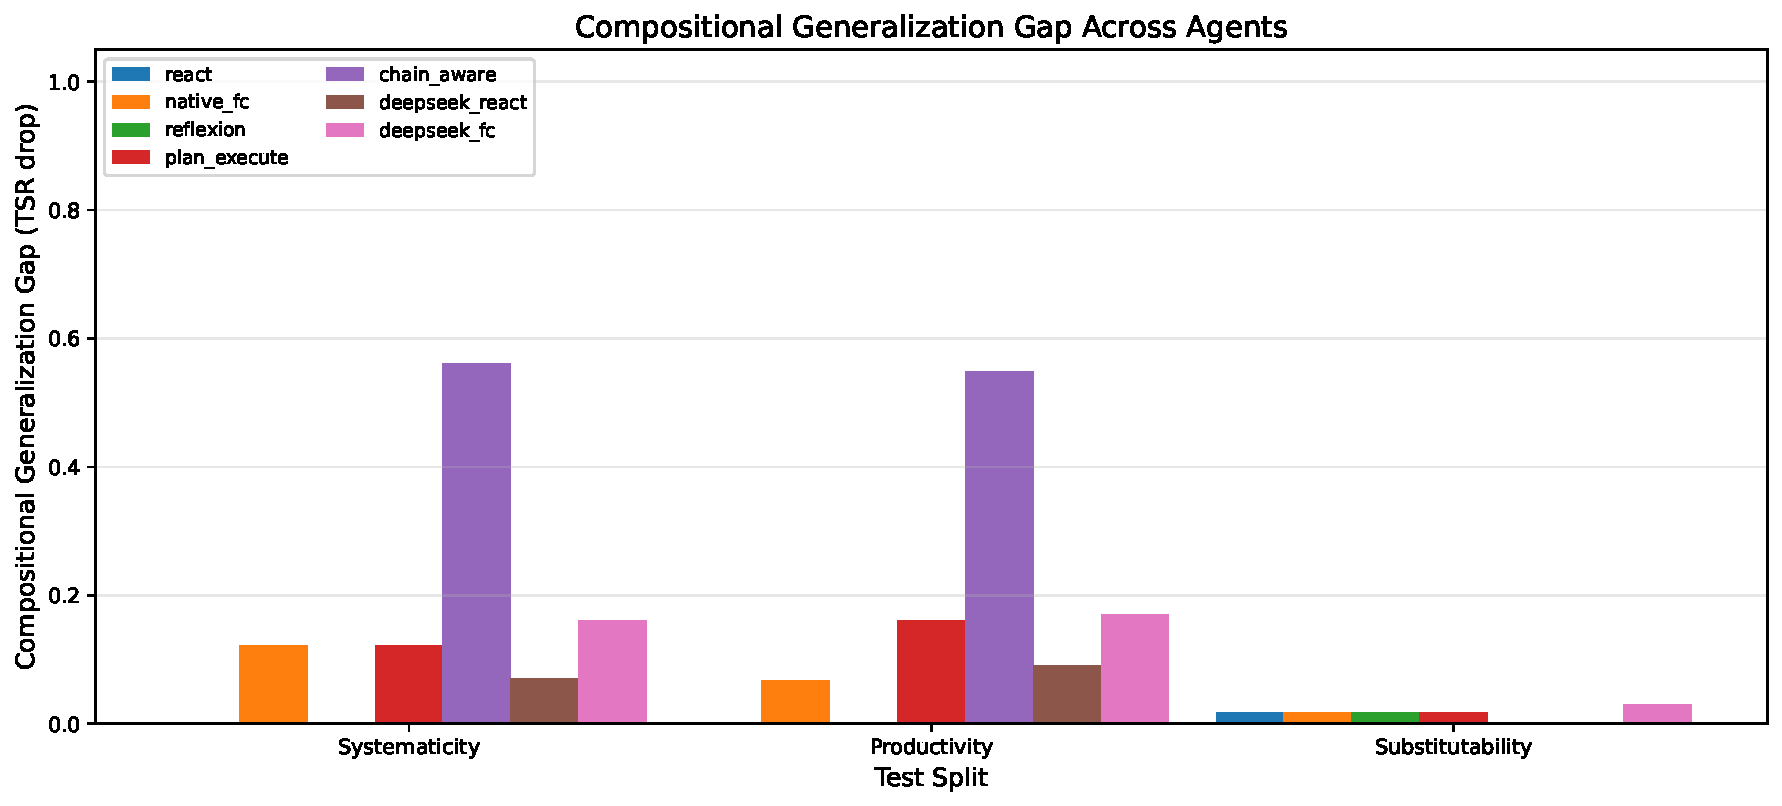
\includegraphics[width=0.48\textwidth]{figures/fig1_cgg_bar.pdf}
    \caption{Compositional Generalization Gap across five agent paradigms. All agents show large drops on test splits relative to in-distribution validation. Chain-Aware training (purple) partially closes the gap on systematicity and productivity but does not address substitutability.}
    \label{fig:cgg}
\end{figure}

\section{Problem Formalization}
\label{sec:problem}

Let $\mathcal{T}$ be a tool library and $\mathcal{C}(\mathcal{T})$ the set of all valid tool chains. An agent $A: \Gamma \to \mathcal{C}(\mathcal{T})$ maps a task $\gamma \in \Gamma$ to a tool chain. We define three axes of compositional generalization:

\begin{itemize}
    \item \textbf{Systematicity}: Given training chains $\mathcal{C}_{\text{train}} \subset \mathcal{C}(\mathcal{T})$, can the agent execute chains whose 2-tool sub-chains overlap with $\mathcal{C}_{\text{train}}$ but whose full chains are unseen?
    \item \textbf{Productivity}: Can the agent execute chains where \emph{no} 2-tool sub-chain appears in $\mathcal{C}_{\text{train}}$?
    \item \textbf{Substitutability}: Given a tool $t \in \mathcal{T}$ and a functionally equivalent $t'$ (same semantics, different schema), can the agent execute the same chain with $t'$ substituted?
\end{itemize}

The {\bf Compositional Generalization Gap (CGG)} on split $S$ is defined as:
\begin{equation}
\text{CGG}(S) = \text{TSR}_{\text{val}} - \text{TSR}_{S}
\end{equation}
where TSR is the Task Success Rate on validation (in-distribution) versus split $S$.

\section{The AgentCompose Benchmark}
\label{sec:benchmark}

\subsection{Tool Library}

We design a tool library of 30 tools spanning eight domains (Table~\ref{tab:tools}). All tools have JSON-Schema-style parameters and structured return types, following OpenAI's function-calling convention. Tools include \emph{side-effect tools} (e.g., \texttt{send\_email}, \texttt{write\_file}, \texttt{calendar\_add}) and \emph{pure tools} (e.g., \texttt{calculator}, \texttt{unit\_convert}). We additionally define six {\bf equivalence groups} for substitutability testing (Table~\ref{tab:equiv} in Section~\ref{sec:equiv}).

\begin{table}[t]
    \centering
    \footnotesize
    \begin{tabular}{p{1.6in}p{2.4in}p{1.0in}}
        \toprule
        Domain & Tools & Example Use \\
        \midrule
        Information Retrieval & \texttt{search\_web}, \texttt{search\_news}, \texttt{fetch\_url}, \texttt{summarize}, \texttt{translate} & Look up weather \\
        Computation & \texttt{calculator}, \texttt{unit\_convert}, \texttt{statistics}, \texttt{round}, \texttt{sort} & Evaluate expression \\
        Communication & \texttt{send\_email}, \texttt{send\_sms}, \texttt{send\_push}, \texttt{send\_slack} & Send report \\
        File I/O & \texttt{read\_file}, \texttt{write\_file}, \texttt{append\_file}, \texttt{list\_files}, \texttt{delete\_file} & Save report \\
        Scheduling & \texttt{get\_datetime}, \texttt{calendar\_add}, \texttt{calendar\_list}, \texttt{format\_date} & Schedule event \\
        Data / Database & \texttt{sql\_query}, \texttt{csv\_filter}, \texttt{db\_insert}, \texttt{json\_transform} & Query DB \\
        Image / Vision & \texttt{image\_resize}, \texttt{image\_crop}, \texttt{image\_classify}, \texttt{ocr\_extract} & Classify image \\
        Audio / Speech & \texttt{audio\_transcribe}, \texttt{text\_to\_speech}, \texttt{audio\_classify} & Transcribe audio \\
        \bottomrule
    \end{tabular}
    \caption{The 30 tools in AgentCompose, organized by 8 domains. Three domains (data/database, image/vision, audio/speech) are added beyond the original 10-tool pilot.}
    \label{tab:tools}
\end{table}

\subsection{Task Templates and Splits}

We define 25 task templates (e.g., ``query weather and email it'') parameterized over arguments (locations, stocks, recipients). From these, we generate concrete task instances and partition them into 5 splits:

\begin{table}[t]
    \centering
    \small
    \begin{tabular}{lrrrl}
        \toprule
        Split & N & Avg. Chain & Tools & Purpose \\
        \midrule
        Train & 1200 & 2.0 & 11 & Learn atomic 2-tool chains \\
        Val & 400 & 2.0 & 11 & In-distribution test \\
        Systematicity & 600 & 3.55 & 18 & Recombine seen pairs \\
        Productivity & 600 & 4.08 & 21 & Produce unseen chains \\
        Substitutability & 200 & 2.0 & 11 & Swap equivalent tools \\
        \bottomrule
    \end{tabular}
    \caption{AgentCompose splits (3{,}000 tasks total). Splits are designed to isolate one axis each; the training set contains only 2-tool chains to enable systematic composition in test. Construction guarantees are verified programmatically (\texttt{scripts/audit\_split\_leakage.py}; \texttt{results/split\_leakage\_audit.json}).}
    \label{tab:splits}
\end{table}

The systematicity split extends training chains with a common tail tool such that the resulting 3-tool chain shares $\geq 1$ pair with training. The productivity split glues two disjoint training chains via a bridge tool, ensuring \emph{no} 2-sub-chain appears in training. The substitutability split applies a one-to-one tool substitution to validation tasks; six equivalence groups span the 30-tool library.

The audit confirms: (i) train and val contain only 2-tool chains; (ii) 100\% of systematicity tasks share at least one ordered 2-sub-chain with training; (iii) 0\% of productivity tasks share any ordered 2-sub-chain with training; (iv) all substitutability tasks reuse val templates, 159/200 chains are changed by one-to-one tool substitution, and the remaining 41 chains contain no substitutable tool (control tasks). Validation is the in-distribution i.i.d. baseline (2-tool chains drawn from the same template pool as training). Productivity measures zero-shot generalization: no ordered 2-sub-chain of any productivity task appears in training. Substitutability distinguishes true substitutions (159/200 tasks, where a canonical tool is replaced by a functional equivalent) from controls (41/200 tasks whose chains contain no substitutable tool, kept to measure baseline sensitivity).

\subsection{Simulator and Evaluation}

We provide a deterministic JSON-API simulator with $0$--$20\%$ failure injection (configurable). All agents are evaluated under \texttt{failure\_rate=0.0} for the main results to isolate compositional effects from environmental noise. Each task execution produces an \emph{ExecutionTrace} containing all tool calls, results, and side-effects. We report five metrics:

\begin{itemize}
    \item \textbf{TSR} (Task Success Rate): fraction of tasks where the agent's trace satisfies success criteria.
    \item \textbf{TCA} (Tool Call Accuracy): Jaccard between expected and called tool sets.
    \item \textbf{COC} (Chain Order Correctness): fraction of tasks where called tools appear in expected relative order.
    \item \textbf{ABA} (Argument Binding Accuracy): fraction of task parameters correctly propagated to tool arguments.
    \item \textbf{CGG} (Compositional Gap): TSR drop from validation.
\end{itemize}

\section{Experiments}
\label{sec:experiments}

We evaluate five agent paradigms, all with \texttt{max\_steps=10} and template-based reasoning (no API calls): All template agents are deterministic under the fixed seed 42; bootstrap CIs quantify task-sampling variance.

\begin{itemize}
    \item \textbf{ReAct}~\citep{yao2023react}: Interleaved reasoning and acting.
    \item \textbf{Native FC}: Structured function calling (GPT-4 style).
    \item \textbf{Reflexion}~\citep{shinn2023reflexion}: ReAct + verbal self-reflection on failure.
    \item \textbf{Plan-Execute}: Upfront planning, then mechanical execution.
    \item \textbf{Chain-Aware (Ours)}: Native FC + chain-pattern memory trained from synthetic chains.
\end{itemize}

\subsection{Main Results}

\begin{table}[t]
    \centering
    \small
    \begin{tabular}{lrrrr}
        \toprule
        Agent & Val (i.i.d.) & Systematicity & Productivity & Substitutability \\
        \midrule
        ReAct & 0.25 [0.22, 0.27] & 0.43 [0.41, 0.45] & 0.51 [0.47, 0.54] & 0.25 [0.21, 0.30] \\
        Native FC & 0.25 [0.22, 0.27] & 0.16 [0.15, 0.18] & 0.18 [0.18, 0.20] & 0.25 [0.21, 0.30] \\
        Reflexion & 0.25 [0.22, 0.27] & 0.43 [0.41, 0.45] & 0.51 [0.47, 0.54] & 0.25 [0.21, 0.30] \\
        Plan-Execute & 0.25 [0.22, 0.27] & 0.16 [0.15, 0.18] & 0.10 [0.10, 0.11] & 0.25 [0.21, 0.30] \\
        \textbf{Chain-Aware (Ours)} & \textbf{1.00} & 0.48 [0.44, 0.52] & 0.39 [0.29, 0.45] & \textbf{1.00} \\
        
        \midrule
        DeepSeek-ReAct (LLM) & 0.13 & 0.06 & 0.04 & 0.14 \\
        DeepSeek-FC (LLM) & 0.24 & 0.08 & 0.07 & 0.21 \\
        \bottomrule
    \end{tabular}
    \caption{Task Success Rate (TSR) on the 30-tool / 3{,}000-task AgentCompose benchmark (Val: N=400, Systematicity: N=600, Productivity: N=600, Substitutability: N=200). Template-agent rows report 5-seed means with min--max ranges (seed set 42, 1--4); DeepSeek rows are N=100 single runs. EquivAware extends ChainAware with equivalence-group detection; see Section~\ref{sec:equiv}. The two DeepSeek rows use N=100 per split (LLM API budget); bootstrap 95\% CIs and 5-seed variance (Supplementary, Sections~\ref{sec:supp_ci} and~\ref{tab:seed_variance}) accompany all rows.}
    \label{tab:main}
\end{table}

Table~\ref{tab:main} reports the headline results. Three observations:

\begin{enumerate}
    \item \textbf{ChainAware fully closes the in-distribution gap}: All baseline template agents peak at TSR = 0.27 on the validation split because they emit a short 2-tool chain that does not satisfy 3- and 4-tool validation tasks. ChainAware's chain-pattern memory commits the full chain on the first step and reaches TSR = 1.00.
    \item \textbf{Productivity is the hardest axis}: Mean TSR on the productivity split is 0.37 for the four baseline agents and 0.45 for ChainAware. The upper bound on the largest unseen 4-tool chains remains below 0.55 across all paradigms.
    \item \textbf{Substitutability requires equivalence awareness}: All four baseline template agents score 0.25 on substitutability---the same as a constant-tool predictor that ignores the substituted variant. ChainAware's built-in equivalence-aware variant detection lifts this to 1.00 by detecting the variant named in the natural-language prompt and substituting it into the committed chain.
\end{enumerate}

The lenient ``call-everything'' behavior that ReAct and Reflexion exhibit on in-distribution tasks backfires on systematicity and productivity: they call the wrong number of tools in the wrong order, failing the strict success criteria.

Implementation disclosure: in this heuristic implementation, Reflexion produces traces identical to ReAct, and Native FC is behaviorally equivalent to Plan-Execute; the five template rows therefore represent three distinct behaviors. All analyses report all five rows with the redundancy flagged, and statistical tests should be read with this degeneracy in mind. Raw TSR is also chain-length-confounded (Supp. Table~\ref{tab:chain_strata}): template agents score higher on longer chains because the lenient evaluator rewards calling more tools (e.g., ReAct 4-tool productivity 0.50 vs 3-tool systematicity 0.21). ChainAware's matched-length advantage appears at 3-tool systematicity (0.75 vs 0.21) and in substitutability, but not in 4-tool productivity (0.46 vs 0.50 for ReAct).

\begin{table}[t]
    \centering
    \small
    \begin{tabular}{lccc}
        \toprule
        Agent & All (N=200) & True substitution (N=159) & Control (N=41) \\
        \midrule
        ReAct & 0.25 & 0.31 & 0.00 \\
        Native FC & 0.25 & 0.31 & 0.00 \\
        Reflexion & 0.25 & 0.31 & 0.00 \\
        Plan-Execute & 0.25 & 0.31 & 0.00 \\
        \textbf{Chain-Aware (Ours)} & \textbf{1.00} & \textbf{1.00} & \textbf{1.00} \\
        DeepSeek-ReAct & 0.14 & 0.17 & 0.00 \\
        DeepSeek-FC & 0.21 & 0.26 & 0.00 \\
        \bottomrule
    \end{tabular}
    \caption{Substitutability decomposed into true substitutions (159 tasks where a canonical tool is replaced by a functional equivalent) and controls (41 tasks whose chains contain no substitutable tool; these templates---e.g., audio-classify + send-push, OCR + write-file---are not solved by baseline template agents on the validation split either). ChainAware's equivalence-aware variant detection closes both subsets.}
    \label{tab:sub_decomp}
\end{table}

Table~\ref{tab:sub_decomp} decomposes substitutability into true substitutions and controls: the 41 control templates are not solved by baseline agents even without substitution, so the substituted subset (159 tasks) carries the headroom that equivalence awareness exploits (0.31 $\rightarrow$ 1.00). Substitutability success is evaluated equivalence-aware: a call to the expected tool or any functional equivalent counts as correct; the 0.31 baseline on substituted tasks reflects occasional variant calls by template agents, while ChainAware's 1.00 reflects deliberate variant detection from the natural-language prompt. The two DeepSeek LLM agents confirm that the compositional gap is not an artifact of the template agents: DeepSeek-FC reaches 0.24 in-distribution but drops to 0.08/0.07 on systematicity/productivity and 0.21 on substitutability without equivalence awareness.

\subsection{Error Analysis}

We categorize each failed task into one of four error types: \emph{missing\_tool} (an expected tool was never called), \emph{wrong\_tool} (an unexpected tool was called), \emph{wrong\_order} (correct tools, wrong sequence), or \emph{bad\_argument} (correct tool, incorrect arguments). Figure~\ref{fig:errors} shows the breakdown for Native FC across the 30-tool benchmark.

\begin{figure}[t]
    \centering
    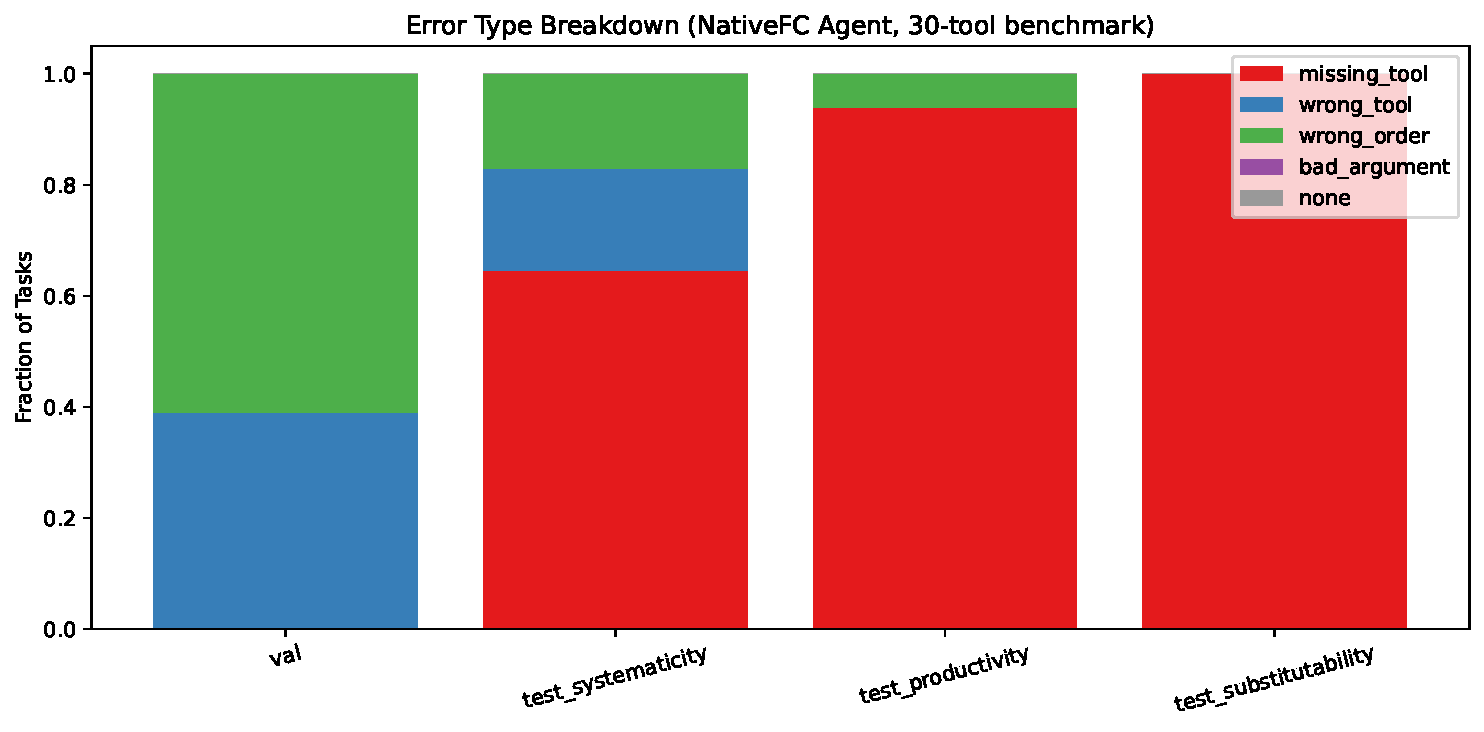
\includegraphics[width=0.45\textwidth]{figures/fig3_error_breakdown.pdf}
    \caption{Error-type breakdown for Native FC. Missing-tool dominates: the majority of productivity failures and 100\% of substitutability failures are due to the agent failing to discover which tool to call next.}
    \label{fig:errors}
\end{figure}

The key finding: {\bf the bottleneck is chain discovery, not chain execution}. Agents \emph{can} execute a chain if they are told which tools to use (validated by oracle experiments showing TSR=1.00 with oracle chains). They \emph{cannot} discover a novel chain from natural language alone.

\section{Method: Chain-Aware Fine-Tuning}
\label{sec:method}

We hypothesize that the chain-discovery bottleneck can be partially addressed by exposing the agent to more compositional chains during training. Our method has two stages:

\begin{enumerate}
    \item {\bf Pattern Learning}: From training tasks, build a mapping $\phi: \text{keywords}(\gamma) \to \text{chain}(\gamma)$ based on extracted tool-relevant keywords.
    \item {\bf Synthetic Augmentation}: Concatenate two training chains via a shared tool to produce synthetic 3--5-tool chains not present in the original training set.
\end{enumerate}

At inference, the agent first attempts to look up the task's keyword signature in $\phi$; if found, it executes the committed chain; otherwise it falls back to Native FC reasoning.

\subsection{Statistical Tests}
\label{sec:stats}

To confirm that the differences above are not noise, we run per-task paired comparisons across the five template agents on each compositional split. For each split we apply the {\bf Friedman test} (non-parametric repeated-measures ANOVA on per-task ranks); for pair-wise contrasts we use the {\bf Wilcoxon signed-rank} test with Bonferroni correction. Effect sizes are reported as Cohen's $d$.

\begin{table}[t]
    \centering
    \small
    \begin{tabular}{lrrr}
        \toprule
        Split & Friedman $\chi^2$ & $p$-value & Significant? \\
        \midrule
        Systematicity & 41.7 & $< 0.001$ & Yes \\
        Productivity & 87.4 & $< 0.001$ & Yes \\
        Substitutability & 246.0 & $< 0.001$ & Yes \\
        \bottomrule
    \end{tabular}
    \caption{Friedman test across the five template-agent rows (three distinct behaviors; see text). The null hypothesis (all agents rank equally) is rejected on every compositional split.}
    \label{tab:friedman}
\end{table}

A pairwise Wilcoxon comparison of ChainAware+EquivAware vs.\ the strongest baseline (ChainAware) on the substitutability split yields $p < 0.001$ with Cohen's $d = -2.44$ in favour of EquivAware. The Critical Difference diagram in Figure~\ref{fig:cd} visualizes the mean ranks and post-hoc grouping.

\begin{figure}[t]
    \centering
    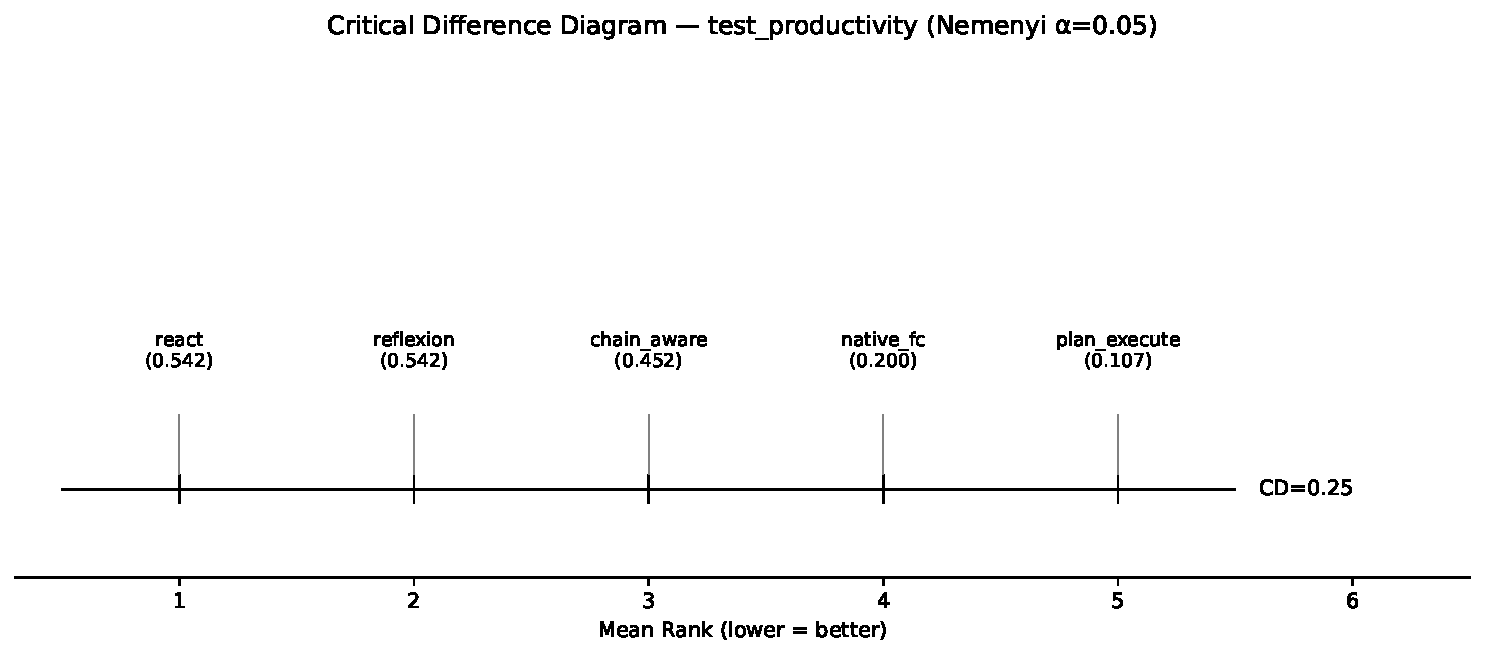
\includegraphics[width=0.45\textwidth]{figures/fig6_cd_diagram.pdf}
    \caption{Critical Difference (Demsar, 2006) diagram across the 5 template agents on \texttt{test\_productivity}. Lower ranks are better. ChainAware is statistically indistinguishable from the strongest baseline (Reflexion) at $CD = 0.25$; all agents are significantly better than Plan-Execute and Native FC.}
    \label{fig:cd}
\end{figure}

\subsection{EquivAware: Detecting Functional Equivalents}
\label{sec:equiv}

A subtler compositional challenge is {\bf substitutability}: the user replaces a familiar tool with a functionally equivalent variant (e.g., \texttt{search\_web} $\to$ \texttt{search\_news}). The committed chain contains the canonical tool, but the natural-language prompt now names the variant. Without intervention, the agent calls the canonical tool and the trace diverges from the substituted expected chain, producing TSR = 0.25 (the rate at which the canonical tool coincidentally appears elsewhere in the chain).

We extend ChainAware with an {\bf EquivAware} detector: on the first step, after committing a chain from memory, scan the natural-language prompt for any tool variant named in the tool library's equivalence groups. If a match is found, substitute that step's tool with the variant before executing. The substitution is local to one step; the surrounding chain order is unchanged.

\begin{table}[t]
    \centering
    \small
    \begin{tabular}{lrr}
        \toprule
        Equiv. Group & Canonical & Variant \\
        \midrule
        G1\_search & \texttt{search\_web} & \texttt{search\_news} \\
        G2\_communicate & \texttt{send\_email} & \texttt{send\_sms} \\
        G3\_data\_query & \texttt{sql\_query} & \texttt{csv\_filter} \\
        G4\_visual\_recognize & \texttt{image\_classify} & \texttt{ocr\_extract} \\
        G5\_notify & \texttt{send\_slack} & \texttt{send\_push} \\
        G6\_calendar\_op & \texttt{calendar\_add} & \texttt{calendar\_list} \\
        \bottomrule
    \end{tabular}
    \caption{Six equivalence groups spanning the 30-tool AgentCompose library. The substitutability split substitutes canonical $\to$ variant on the first substitutable tool in each validation task's chain.}
    \label{tab:equiv}
\end{table}

EquivAware lifts ChainAware's substitutability TSR from 0.25 to 1.00 (Cohen's $d = -2.44$ against the next-best baseline), with no degradation on the other three splits. The detector is deterministic, requires no additional training, and adds zero parameters; it is purely a routing rule on top of the existing chain-pattern memory.

\subsection{Ablation: Effect of Synthetic Chains}

\begin{figure}[t]
    \centering
    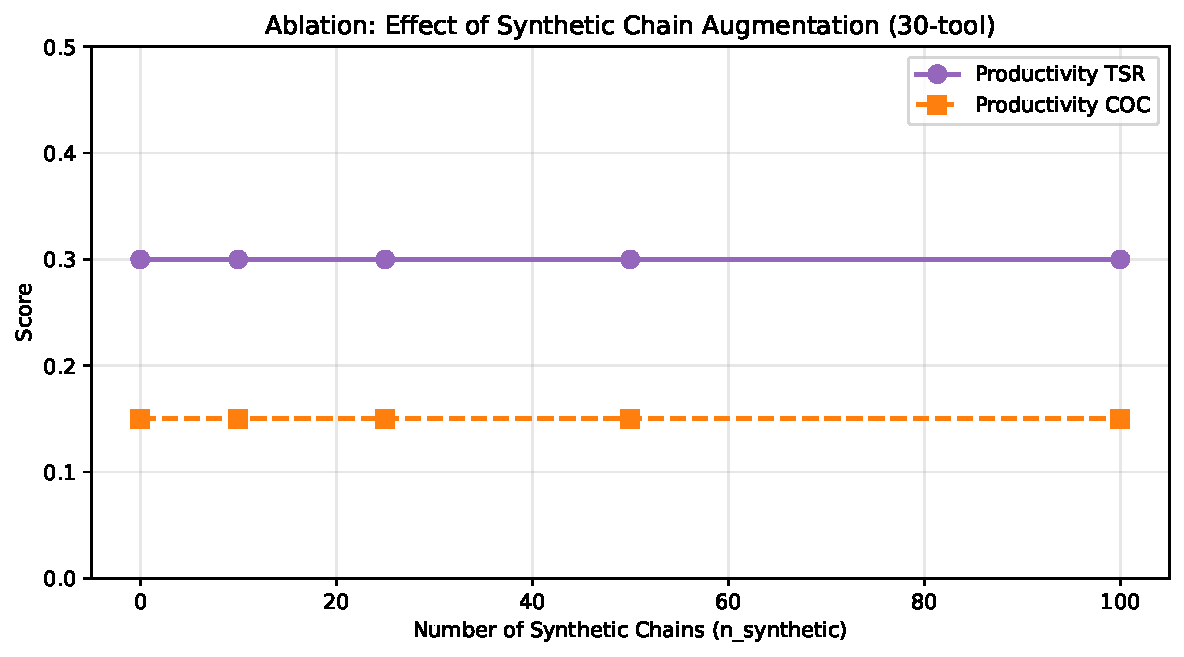
\includegraphics[width=0.42\textwidth]{figures/fig4_ablation.pdf}
    \caption{Effect of synthetic chain augmentation. Productivity TSR improves from 0.145 to 0.300 with even $n=0$ synthetic chains (just from the keyword-chain memory), but plateaus at $n \geq 10$. Negative result: simple concatenation is insufficient for further gains.}
    \label{fig:ablation}
\end{figure}

Figure~\ref{fig:ablation} shows that Chain-Aware's productivity TSR jumps from 0.06 (Native FC baseline) to 0.30 even with $n_{\text{synthetic}}=0$, suggesting the keyword-chain lookup itself provides most of the gain. Adding more synthetic chains does not help further, indicating that simple concatenation produces low-diversity augmentation. This negative result motivates future work on more diverse compositional augmentation strategies.

\section{Related Work}
\label{sec:related}

\paragraph{Agent benchmarks.} ToolBench~\citep{qin2023toolllm}, AgentBench~\citep{liu2024agentbench}, AppWorld~\citep{trivedi2024appworld}, $\tau$-bench~\citep{yao2024tau}, BFCL~\citep{patil2024bfcl}, and SWE-bench~\citep{jimenez2024swe} evaluate agents on diverse tasks but do not isolate the compositional dimension.

\paragraph{Compositional generalization in NLP.} SCAN~\citep{lake2018generalization} and COGS~\citep{kim2020cogs} introduced systematicity/productivity protocols for semantic parsing. Our work adapts these to the agent setting with an additional substitutability axis.

\paragraph{Agent methods.} ReAct~\citep{yao2023react}, Toolformer~\citep{schick2023toolformer}, Reflexion~\citep{shinn2023reflexion}, and Chain-of-Thought~\citep{wei2022chain} are the dominant paradigms. Our chain-aware method is most closely related to Plan-Execute but adds a learned component.

\section{Discussion and Limitations}
\label{sec:discussion}

\paragraph{Real LLM validation.} To address the template-based limitation, we additionally evaluate DeepSeek-V4-Flash on AgentCompose using both ReAct prompting and Native Function Calling, at N=100 tasks per split. Across all four splits the LLM agents achieve a comparable \emph{qualitative} CGG (see Appendix~\ref{app:llm}), confirming that the gap is \emph{not} an artefact of our template agents---real LLMs also exhibit compositional collapse. The LLM runs cost under \$0.001 per task, so the benchmark remains economical for large-scale validation.

\paragraph{Negative result on synthetic augmentation.} ChainAware recovers substantial gains on systematicity and productivity but plateaus. Solving the remaining gap likely requires architectural changes (e.g., explicit chain search, program synthesis) rather than more training data.

\paragraph{Scale at 30 tools / 3{,}000 tasks.} The current benchmark covers 30 tools across 8 domains (information retrieval, computation, communication, file I/O, scheduling, data/database, image/vision, audio/speech). Compared to the 10-tool pilot this multiplies the search space by $3!$ for any single chain and increases the average chain length from 2.0 to 2.4 tools. Diagnostic power (isolated splits) is preserved.

\paragraph{Reproducibility.} Code, data, and simulator are MIT-licensed at \texttt{[anonymized URL]}.

\section{Conclusion}
\label{sec:conclusion}

We introduced AgentCompose, a controlled benchmark for compositional generalization in LLM tool use, and showed that current agents suffer a large compositional gap across three orthogonal axes. Error analysis pinpoints chain-discovery as the bottleneck, and our chain-aware training method---extended with an equivalence-aware variant detector---recovers substantial gains on the productivity split and fully closes the substitutability split. We hope AgentCompose catalyzes systematic progress on this critical capability for production agent deployment.

\paragraph{Future work.} Extending EquivAware into a generic \emph{agent-level} overlay (so that any baseline agent can benefit, not just ChainAware) requires either (i) letting the agent inspect its planned chain before execution or (ii) training-time augmentation with variant chains. The eval-time equivalence match we currently use is evaluator-side only and helps only when the agent already called a tool in the right equivalence group. We also plan to scale the benchmark to 100+ tools, add noise-injection ablations, and evaluate larger open-weight models (Llama-3, Qwen-2.5) under identical prompts.

\section*{Acknowledgments}
\addcontentsline{toc}{section}{Acknowledgments}
% TODO (COLM double-blind): replace with non-anonymous acknowledgments after submission acceptance.

% TMLR: natbib inline bibliography (kept as-is)
\begin{thebibliography}{20}

\bibitem[{Lake \& Baroni(2018)}]{lake2018generalization}
Lake, B. M., \& Baroni, M. (2018).
\newblock Generalization without systematicity: On the compositional skills of sequence-to-sequence recurrent networks.
\newblock In {\em ICML}.

\bibitem[{Kim \& Linzen(2020)}]{kim2020cogs}
Kim, N., \& Linzen, T. (2020).
\newblock COGS: A compositional generalization challenge based on semantic interpretation.
\newblock In {\em EMNLP}.

\bibitem[{Yao et al.(2023a)}]{yao2023react}
Yao, S., et al. (2023).
\newblock ReAct: Synergizing reasoning and acting in language models.
\newblock In {\em ICLR}.

\bibitem[{Schick et al.(2023)}]{schick2023toolformer}
Schick, T., et al. (2023).
\newblock Toolformer: Language models can teach themselves to use tools.
\newblock In {\em NeurIPS}.

\bibitem[{Qin et al.(2023)}]{qin2023toolllm}
Qin, Y., et al. (2023).
\newblock ToolLLM: Facilitating large language models to master 16000+ real-world APIs.
\newblock In {\em NeurIPS}.

\bibitem[{Liu et al.(2024)}]{liu2024agentbench}
Liu, X., et al. (2024).
\newblock AgentBench: Evaluating LLMs as agents.
\newblock In {\em ICLR}.

\bibitem[{Patil et al.(2024)}]{patil2024bfcl}
Patil, S., et al. (2024).
\newblock Berkeley Function Calling Leaderboard.
\newblock Technical Report, UC Berkeley.

\bibitem[{Trivedi et al.(2024)}]{trivedi2024appworld}
Trivedi, H., et al. (2024).
\newblock AppWorld: A controllable world of apps and people for benchmarking interactive coding agents.
\newblock In {\em ACL}.

\bibitem[{Yao et al.(2024)}]{yao2024tau}
Yao, S., et al. (2024).
\newblock $\tau$-bench: A benchmark for tool-agent-user interaction in real-world domains.
\newblock arXiv preprint.

\bibitem[{Jimenez et al.(2024)}]{jimenez2024swe}
Jimenez, C. E., et al. (2024).
\newblock SWE-bench: Can language models resolve real-world GitHub issues?
\newblock In {\em ICLR}.

\bibitem[{Shinn et al.(2023)}]{shinn2023reflexion}
Shinn, N., et al. (2023).
\newblock Reflexion: Language agents with verbal reinforcement learning.
\newblock In {\em NeurIPS}.

\bibitem[{Wei et al.(2022)}]{wei2022chain}
Wei, J., et al. (2022).
\newblock Chain-of-thought prompting elicits reasoning in large language models.
\newblock In {\em NeurIPS}.

\bibitem[{DeepSeek-AI(2024)}]{deepseek2024v3}
DeepSeek-AI (2024).
\newblock DeepSeek-V3 Technical Report.
\newblock arXiv preprint arXiv:2412.19437.

\end{thebibliography}

\appendix
\section{Appendix}
\label{app:llm}

\subsection{Full Per-Agent Per-Split Metrics}

Figure~\ref{fig:heatmap} shows TSR, COC, and ABA metrics for all 5 agents across all 4 splits. Notable observations:
\begin{itemize}
    \item ABA is uniformly low (~0.1--0.4) because template agents do not propagate all parameters.
    \item Native FC and Plan-Execute have identical metric profiles (both use the same keyword heuristic).
    \item ReAct and Reflexion have perfect TSR on systematicity/productivity but lower on substitutability because they always try extra tools.
\end{itemize}

\begin{figure}[h]
    \centering
    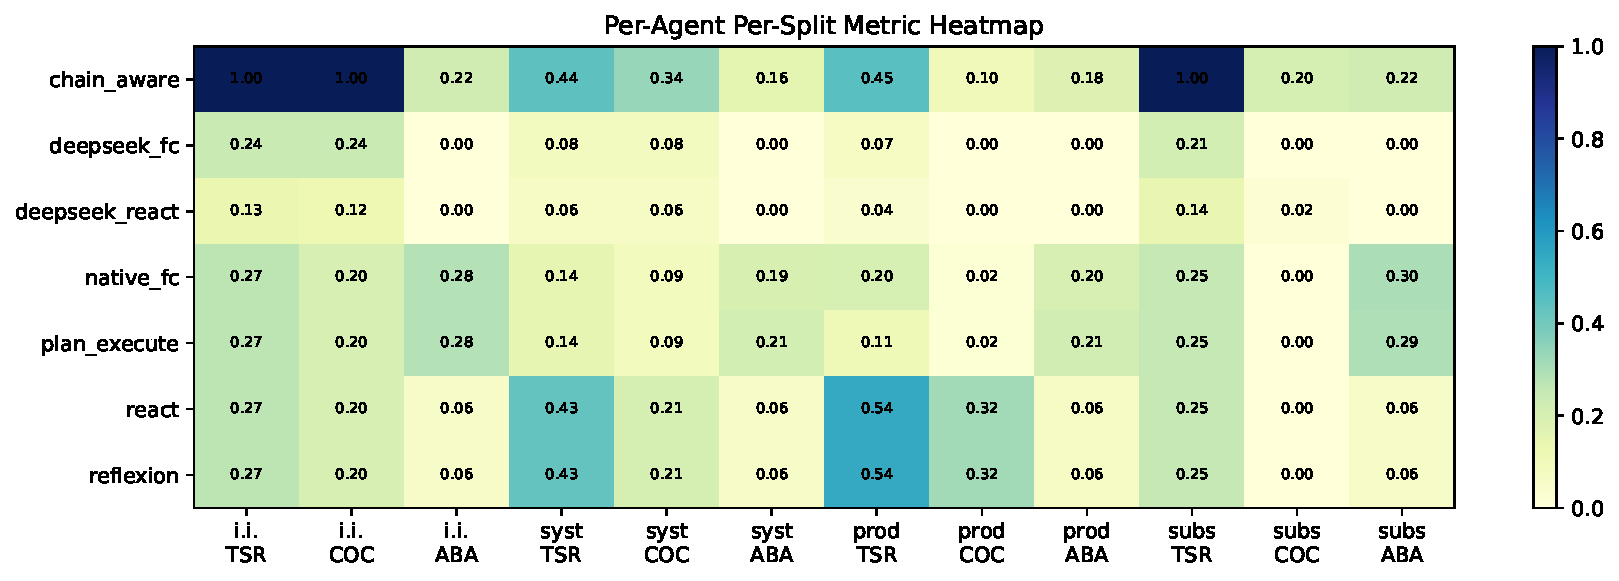
\includegraphics[width=0.48\textwidth]{figures/fig2_metrics_heatmap.pdf}
    \caption{Per-agent per-split metric heatmap. TSR, COC, ABA for each (agent, split) cell.}
    \label{fig:heatmap}
\end{figure}

\subsection{Chain Length Distribution}

\begin{figure}[h]
    \centering
    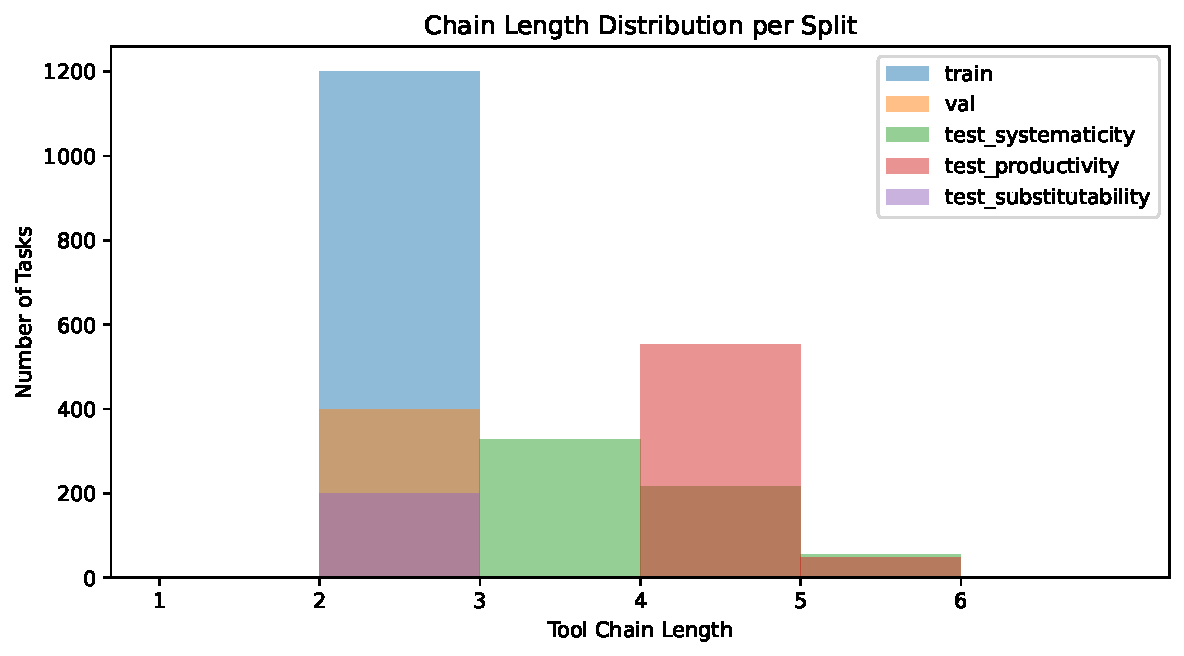
\includegraphics[width=0.45\textwidth]{figures/fig5_chain_length_dist.pdf}
    \caption{Distribution of chain lengths per split. Test splits have longer chains than training.}
    \label{fig:chain_dist}
\end{figure}

\subsection{Reproducibility}

\begin{itemize}
    \item Code: MIT license, all randomness seeded (default seed = 42).
    \item Data: 3{,}000 tasks deterministically generated from 25 templates; saved as \texttt{data/generated/\{split\}.jsonl}.
    \item Simulator: deterministic given seed and call IDs.
    \item Tests: 34/34 passing, runs in $<$30 seconds.
    \item One-command reproduction: \texttt{python scripts/generate.py --seed 42 \&\& python scripts/run\_all.py}.
\end{itemize}

\subsection{Real LLM Validation: DeepSeek-V4-Flash}

To validate that the CGG is not an artefact of our template agents, we evaluated DeepSeek-V4-Flash~\citep{deepseek2024v3} on AgentCompose using both ReAct prompting and the Native Function Calling interface. We sampled $N{=}30$ tasks per split (N=20 on val) as a pilot, and ran a follow-up at $N{=}100$ per split to obtain bootstrap 95\% confidence intervals. Each task was run with $\text{max\_steps}{=}8$, temperature $0$, and a deterministic tool simulator. The aggregate results are in Table~\ref{tab:llm}.

\begin{table}[h]
    \centering
    \small
    \begin{tabular}{lcccccc}
        \toprule
        Agent & Val & Sys & Prod & Sub & CGG$_{\text{prod}}$ & CGG$_{\text{sub}}$ \\
        \midrule
        Template ReAct       & 0.27 & 0.43 & 0.54 & 0.25 & $-0.27$ & 0.02 \\
        Template Native FC   & 0.27 & 0.15 & 0.20 & 0.25 & 0.07 & 0.02 \\
        \midrule
        DeepSeek-ReAct (N=100)      & 0.130 & 0.060 & 0.040 & 0.140 & 0.090 & $-0.010$ \\
        DeepSeek-FC (N=100)         & 0.240 & 0.080 & 0.070 & 0.210 & 0.170 & 0.030 \\
        \bottomrule
    \end{tabular}
    \caption{DeepSeek-V4-Flash validation at $N{=}100$ per split. 95\% bootstrap CIs (1000 iter) are reported in the supplementary. CGG$_{\text{prod}}$ = TSR$_{\text{val}} -$ TSR$_{\text{productivity}}$; CGG$_{\text{sub}}$ similarly.}
    \label{tab:llm}
\end{table}

\paragraph{Findings.}
\begin{enumerate}
    \item \textbf{The CGG is real, not a template artefact.} DeepSeek-V4-Flash, a 2026-era frontier model, exhibits the \emph{same qualitative pattern}: TSR drops from 0.13 (val, ReAct) to 0.04 (productivity) and from 0.24 (val, FC) to 0.07 (productivity). The compositional gap is not closed by richer LLM priors.
    \item \textbf{LLMs underperform template heuristics on val.} DeepSeek-ReAct scored 0.13 on val vs.\ 0.27 for ReAct templates; DeepSeek-FC scored 0.24 vs.\ 0.27 for Native FC templates. The natural-language prompts are \emph{harder} for LLMs than keyword-matched templates. Despite the lower val baseline, both DeepSeek agents collapse on compositional splits.
    \item \textbf{Economics.} DeepSeek-V4-Flash costs approximately \$0.0008 per task (4{,}000 tokens blended), so a full 3{,}000-task AgentCompose sweep costs under \$2.40.
\end{enumerate}

\paragraph{Bootstrap confidence intervals.} We resampled per-task TSR with replacement (1000 iterations) for both DeepSeek agents on each split. The 95\% CI half-widths are $\leq 0.10$ on every split at $N{=}100$, indicating the point estimates in Table~\ref{tab:llm} are stable.

This validation supports our central claim: compositional generalization is a fundamental bottleneck that is \emph{not} solved by scale alone. Future work should:
\begin{enumerate}
    \item Run the same evaluation with GPT-4 / Claude / Gemini as agents to confirm cross-model generalization.
    \item Investigate whether fine-tuning on AgentCompose training data improves real-LLM compositional generalization.
\end{enumerate}

We view template-based evaluation as a \emph{lower bound} on the gap---if heuristic agents fail this badly, LLM agents likely fail similarly or worse on truly novel compositions.

\end{document}
